\documentclass[10pt,a4paper]{article}
\usepackage[utf8]{inputenc}
\usepackage[french]{babel}
\usepackage{float}
\usepackage{amsmath}
\usepackage{graphicx}
\usepackage[left=2cm,right=2cm,top=2cm,bottom=2cm]{geometry}

\author{Jérôme Hue, Damien Carreau}
\title{Traitement du signal - Compte rendu}

\begin{document}
\maketitle
\section{La fonction Transformée de Fourrier Discrète}
\noindent
Données : \\
On échantillone la fonction entre $a$  = -50 secondes et $b$ = 50 secondes, avec un total de $N$ = 32768 échntillons.\\
La période d'échantillonage est : \( T_e = \dfrac{(b-a)}{N} = \dfrac{1}{327,68} \ = 3,1 ms \)  \\
La fréquence d'échantillonage est : \( f_e = \dfrac{1}{T_e} = 327,68 Hz \) \\
L'intervalle entre deux échantillons en fréquence est de fe/N = 1/100.\\

\noindent
Applications : \\
On créer toutes les fonctions données et on affiche leurs spectres. Suivant les spectres sont réels, imaginaires ou nuls.
Pour chaque fonction, on vérifie qu'elle est bien construite en utilisant la fonction inverse de fourrier fournie afin de retomber sur la courbe initiale.\\

Pour toutes les fonctions, on prend : $f = 0.01 Hz$\\


\begin{figure}[h]
\begin{center}
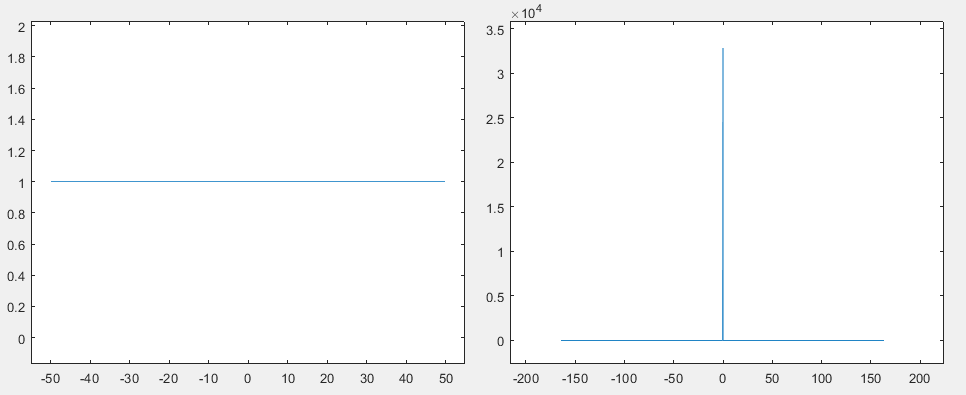
\includegraphics[scale=0.7]{x0.png}
\caption{$x_0(t) = 1$ - Fonction initiale(gauche) - Partie réelle de la transformée de Fourrier(droite)}
\end{center}
\end{figure} 

\begin{figure}[h]
\begin{center}
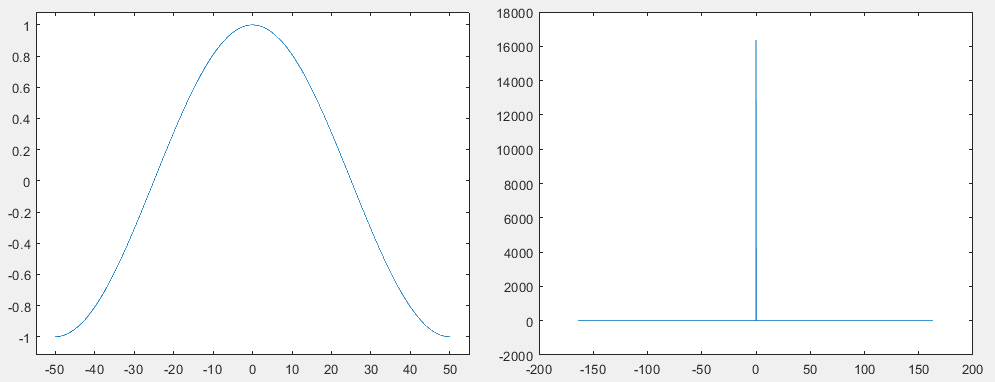
\includegraphics[scale=0.7]{x1.png}
\caption{$x_1(t) = cos(2 \pi f t)$ - Fonction initiale(gauche) - Partie réel de la transformée de Fourrier(droite)}
\end{center}
\end{figure}

\newpage
Fonction ;\\	
\begin{figure}[!h]
\begin{center}
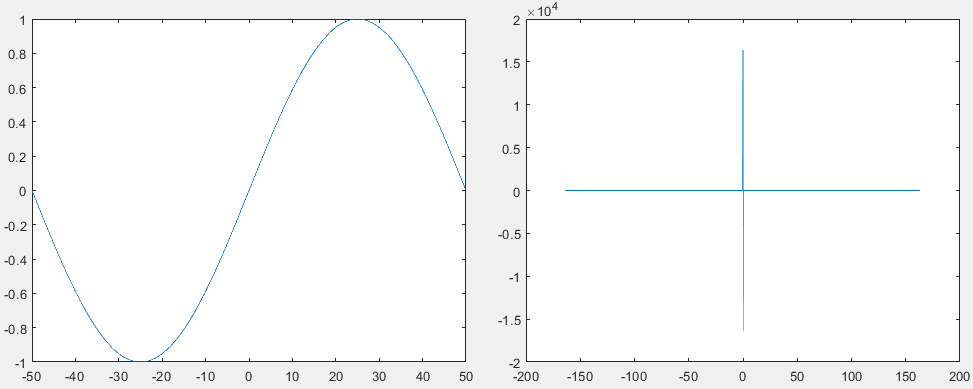
\includegraphics[scale=0.7]{x2_imag.png}
\caption{$x2(t) = sin(2\pi ft)$ - Fonction initiale(gauche) - Partie imaginaire de la transformée de Fourrier(droite)}
\end{center}
\end{figure}


\begin{figure}[h]
\begin{center}
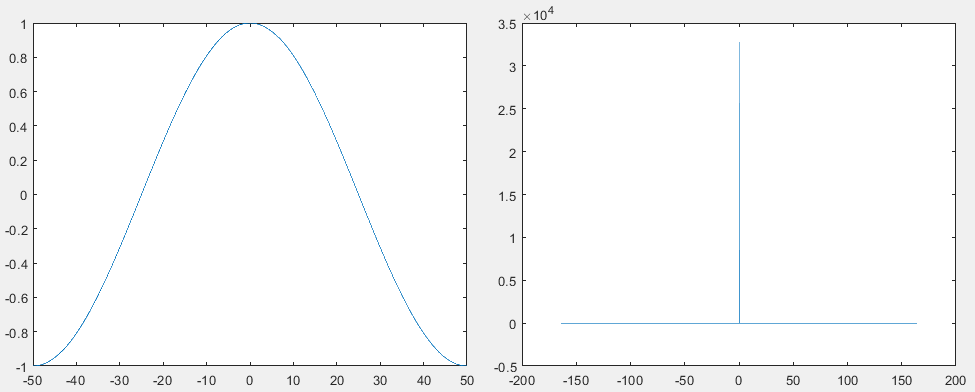
\includegraphics[scale=0.7]{x3.png}
\caption{$x_3(t) = exp(i2\pi ft)$ - Fonction initiale(gauche) - Partie réelle de la transformée de Fourrier(droite)}
\end{center}
\end{figure}

\begin{figure}[h]
\begin{center}
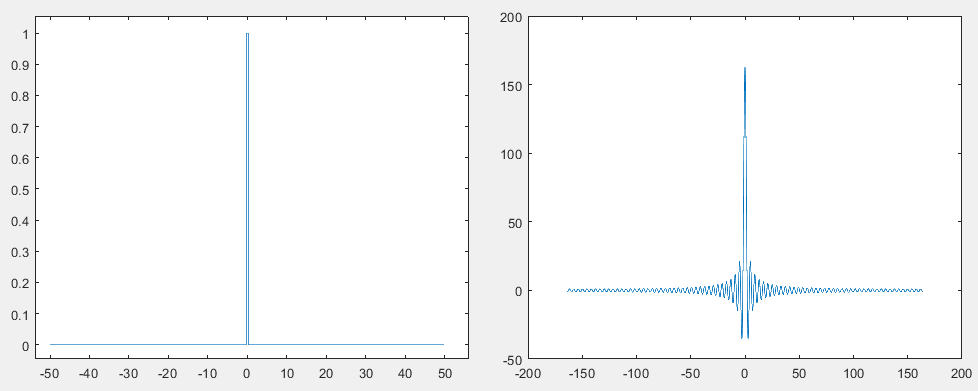
\includegraphics[scale=0.7]{x4.png}
\caption{$x4(t) = (rect_{0.5}(t)$ Fonction initiale(gauche) - Partie réelle de la transformée de Fourrier(droite)}
\end{center}
\end{figure}


\begin{figure}[!h]
\begin{center}
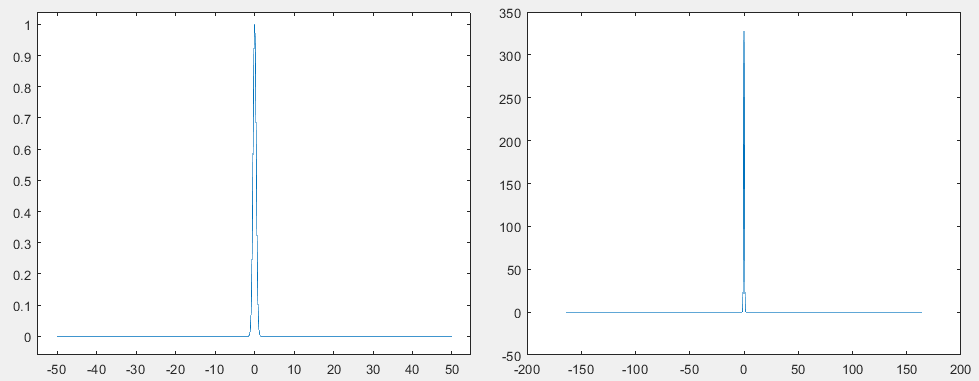
\includegraphics[scale=0.7]{x5.png}
\caption{$x5(t) = exp(\pi*t)$ - Fonction initiale(gauche) - Partie réel de la transformée de Fourrier(droite)}
\end{center}
\end{figure}

\begin{figure}[H]
\begin{center}
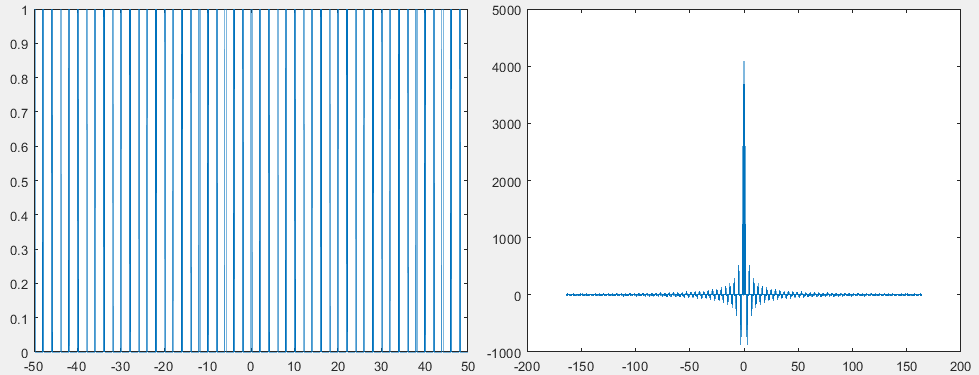
\includegraphics[scale=0.7]{x6.png}
\caption{$x6(t) = mod(rect_{0.5},2)$ - Fonction initiale(gauche) - Partie réel de la transformée de Fourrier(droite)}
\end{center}
\end{figure}

\begin{figure}[H] \begin{center}
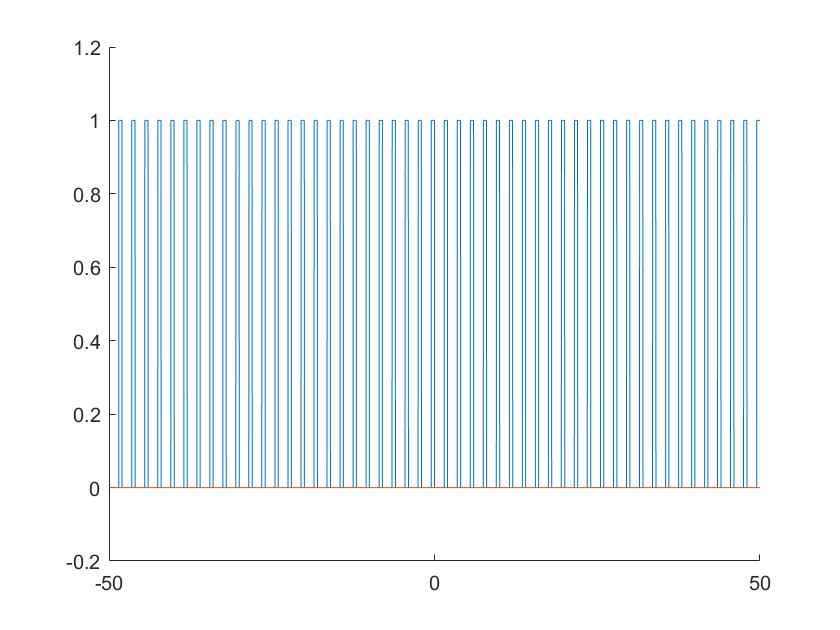
\includegraphics[scale=0.35]{fct6.jpg}
\caption{La fonction 6 après transformée de fourrier inverse}
\end{center} \end{figure}


\newpage
\bigskip
\section{Transmission par modulation d'amplitude}
Dans cette partie, on s'intéresse à deux signaux s1 et s2. On suppose que l'on doit les transmettre. Pour cela on effectue une modulation des signaux comme suit :\\
$c(t) = s1(t)*cos(2 \pi f_1 t)+ s2(t)*cos(2 \pi f_2 t)$\\
\textit(Calcul théorique)

\textit{Comment extraire $s1(t)$ ou $s2(t)$ ?}\\
Pour extraire s1 ou s2 \textit{(figure~\ref{s1s2})}, il faut démoduler le signal c(t) \textit{(figure~\ref{c})} en le multipliant par $cos(2 \pi f_x t)$.(Où $f_x$ correspond à la fréquence de modulation du signal que l'on souhaite démoduler) On calcul ensuite le spectre du ce nouveau signal : $d(t)$ \textit{(figure~\ref{d})} puis on applique un filtre pour récupérer le spectre de $s_x$. On calcul ensuite la transformée inverse pour récupérer le vrai signal \textit{(figure~\ref{s1demod})}.

\begin{figure}[h]
\begin{center}
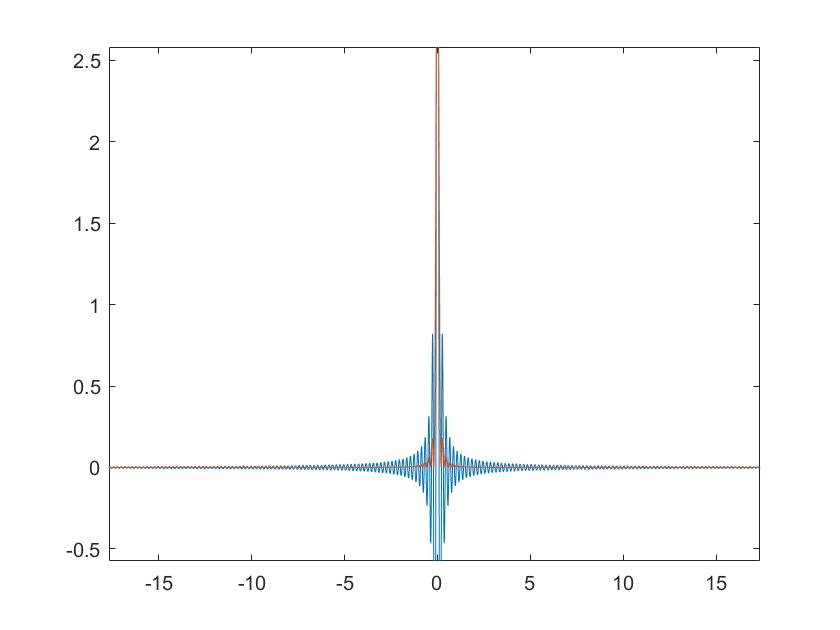
\includegraphics[scale=0.35]{tf_2signaux.jpg}
\caption{Les signaux $s1(t)$  en bleu et $s2(t)$ en orange}
\label{s1s2}
\end{center}
\end{figure}


\begin{figure}	\begin{center}
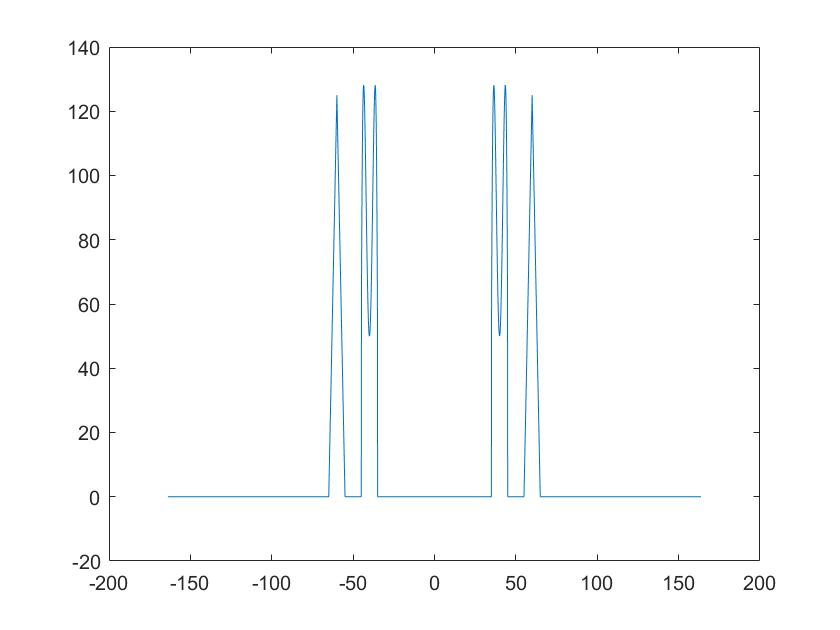
\includegraphics[scale=0.35]{tf_fctc.jpg}
\caption{Le signal $c(t)$. On peut remarquer que $f_1(t)$ = 40 Hz et $f_2(t)$ = 60Hz}
\label{c}
\end{center}	\end{figure}

\begin{figure}	\begin{center}
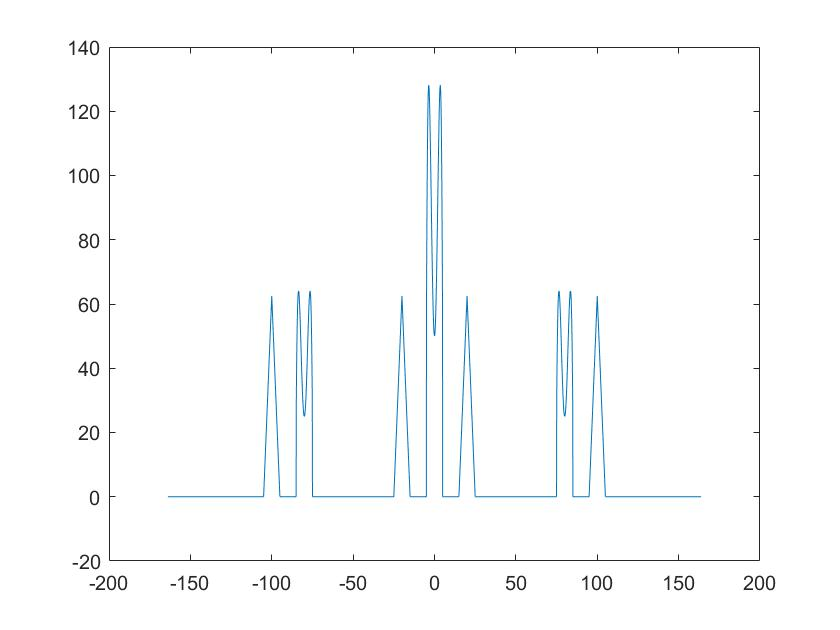
\includegraphics[scale=0.35]{Signal_d.jpg}
\caption{Le signal $d(t)$. On a démodulé le signal $c(t)$ avec $f_1(t)$}
\label{d}
\end{center}	\end{figure}

\begin{figure}	\begin{center}
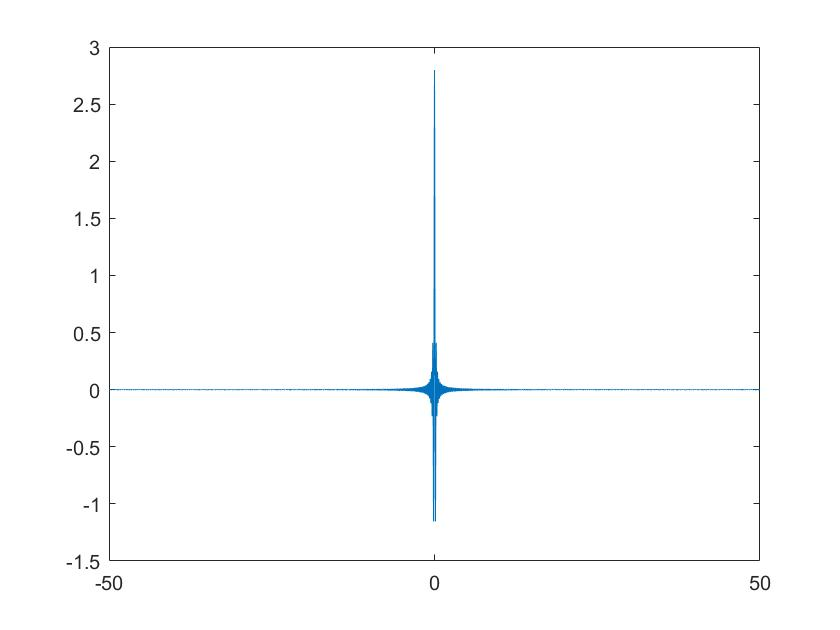
\includegraphics[scale=0.35]{s1_demodule.jpg}
\caption{Le signal $s1(t)$  obtenu après démodulation}
\label{s1demod}
\end{center}	\end{figure}



Pour la démodulation, il faut faire attention à ne pas prendre des fréquence $f_i$ et $f_j$ qui soient trop proches.




\newpage

\section{Échantillonnage et aliasing	}

Ici, on va s'intéresser au signal suivant :
$g_f(t) = s1(t)*sin(2 \pi f t)$\\
On va échantillonner ce signal pour différente valeur de f.\\
Le signal s1 utilisé ici est le même que dans la partie précédente(fourni par l'enseignant).
Par la multiplication du signal par le sinus, on obtient une transformée de fourrier imaginaire. Le spectre de s1 est dédoublé en 2 signaux inverses. Un positif centré en -f et un négatif centré en f.

\begin{figure}[H]	\begin{center}
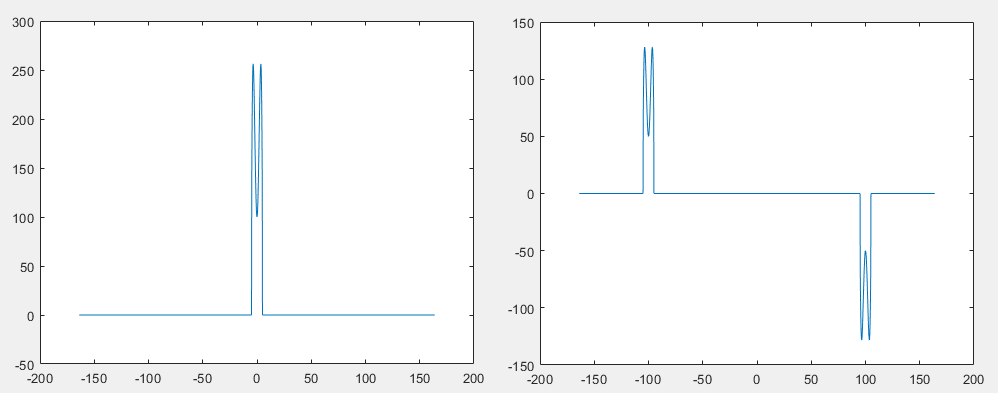
\includegraphics[scale=0.6]{aliasing1.png}
\caption{Transformée réel de s1(gauche) et Transformée imaginaire de $g_{100}$(droite)}
\label{XX}
\end{center}	\end{figure}

Dans l'application développé en classe, notre affichage fréquentiel se fait sur l'intervalle [-163.84;163.83]. Par conséquent, lorsque la fréquence f se rapproche ou dépasse cette l'une des bornes de cette plage, notre affichage n'est plus valide.

\begin{figure}[H]	\begin{center}
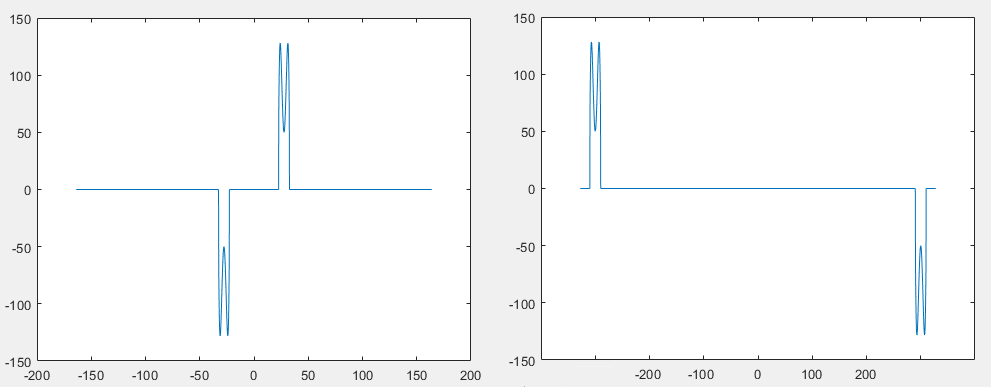
\includegraphics[scale=0.6]{aliasing2.png}
\caption{Transformée de $g_{300}$ par l'application(gauche) et Transformée de $g_{300}$ théorique(droite)}
\label{XX}
\end{center}	\end{figure}

\section{Filtrage}

On va filtrer des images avec le filtre fréquentiel suivant
\[
	H(u,v) = exp(-K((u)^2+(v)^2))
\]
On charge l'image, on en déduit la transformée de Fourrier. Puis on applique le filtre pour chaque pixels. On récupère, pour finir, la transformée inverse de ce résultat.

\begin{figure}[H]	\begin{center}
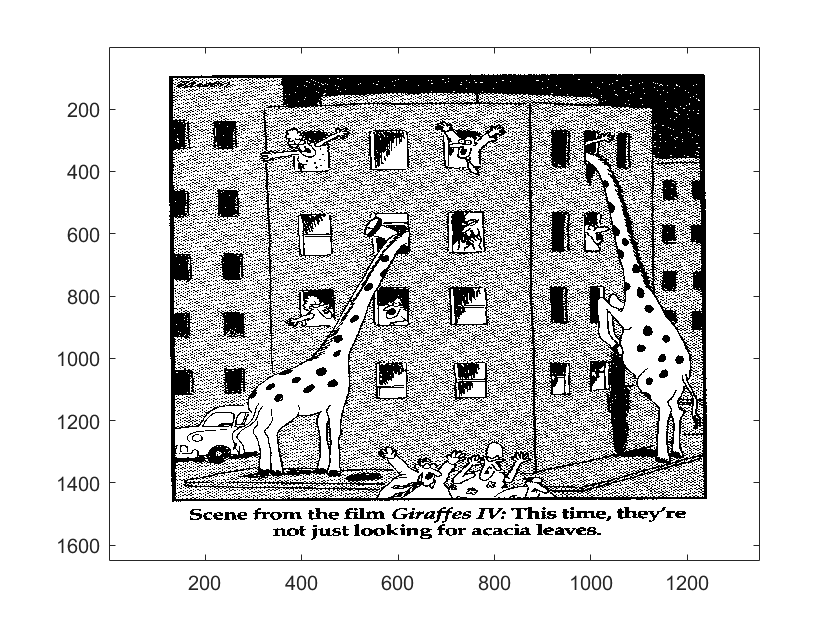
\includegraphics[scale=0.35]{girafe_originale.png}
\caption{L'image originale}
\label{XX}
\end{center}	\end{figure}



\begin{figure}[H]	\begin{center}
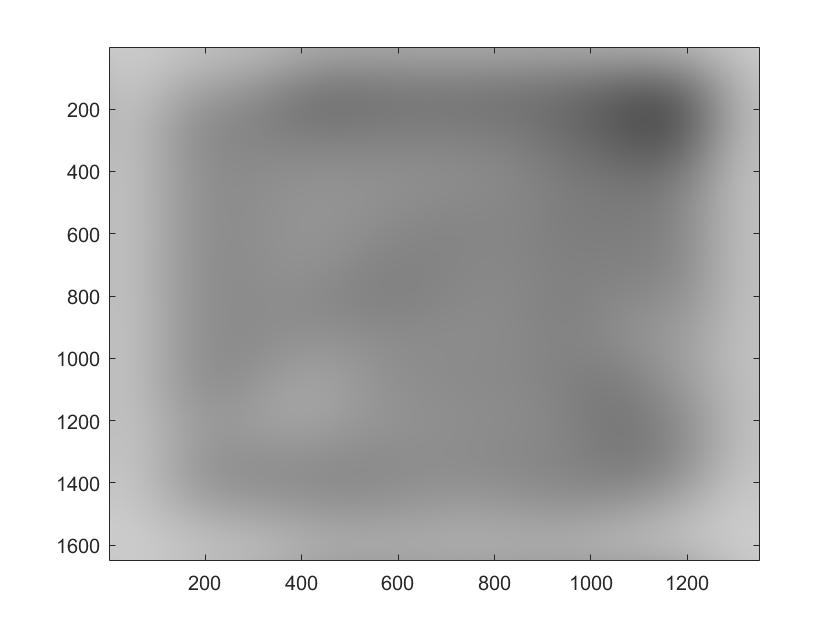
\includegraphics[scale=0.35]{imfiltree_k=0.1.jpg}
\caption{Filtrage avec K=0.1}
\label{XX}
\end{center}	\end{figure}

\begin{figure}[H]	\begin{center}
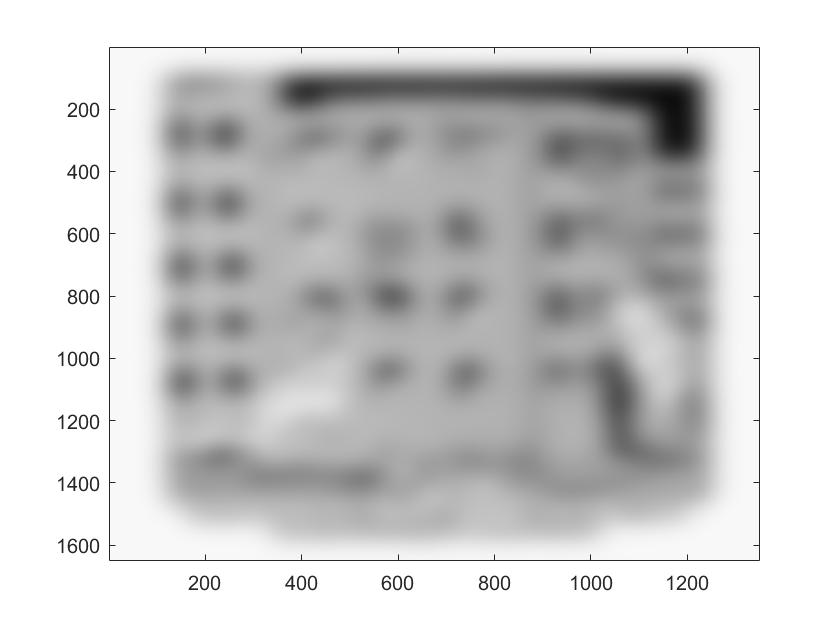
\includegraphics[scale=0.35]{imfiltree_k=0.01.jpg}
\caption{Filtrage avec K=0.01}
\label{XX}
\end{center}	\end{figure}

\begin{figure}[H]	\begin{center}
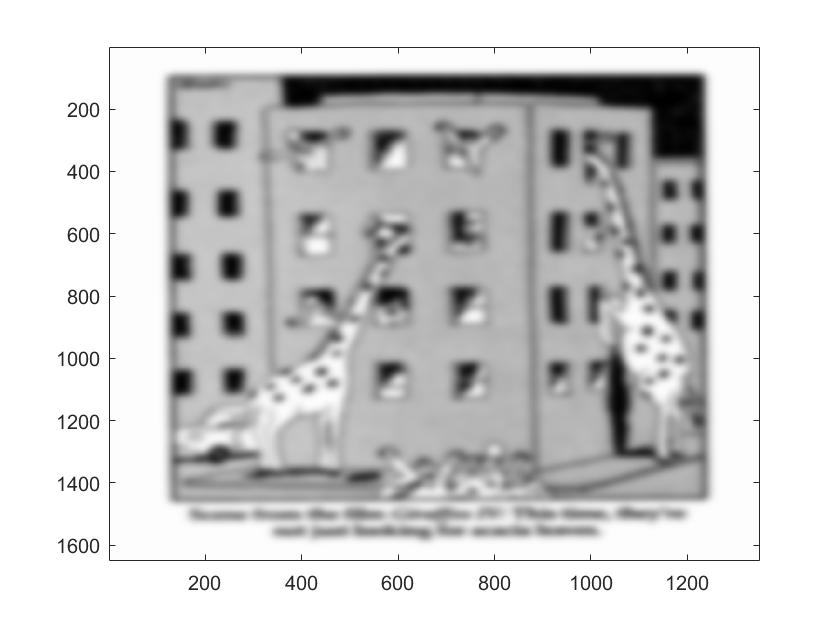
\includegraphics[scale=0.35]{imfiltree_k=0.001.jpg}
\caption{Filtrage avec K=0.001}
\label{XX}
\end{center}	\end{figure}

\subsection{Application}

On veut diviser par 4 la dimension de l'image "girafeIV.jpg". Pour cela, on construit une première image en prenant un point sur 4 dans l’image (en ligne et en colonne).


\begin{figure}[H]	\begin{center}
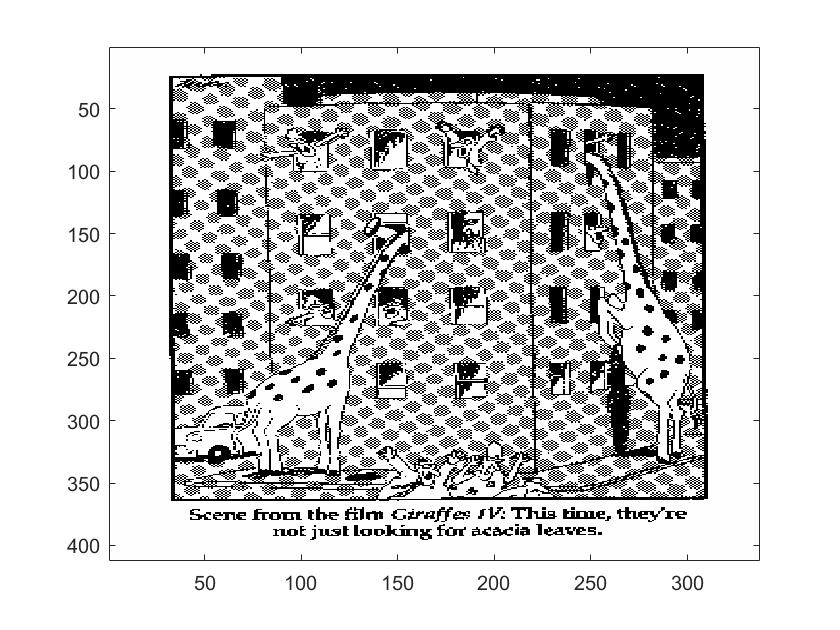
\includegraphics[scale=0.35]{girafe_reduite.jpg}
\caption{L'image réduite en prenant un pixel sur 4 toutes les 4 lignes}
\label{XX}
\end{center}	\end{figure}


On constate une forte dégradation de l'image observée. Pour pallier à cette dégradation, on va filtrer l'image avec le filtre H, puis prendre un point sur 4 de cette image filtrée.

\begin{figure}[H]	\begin{center}
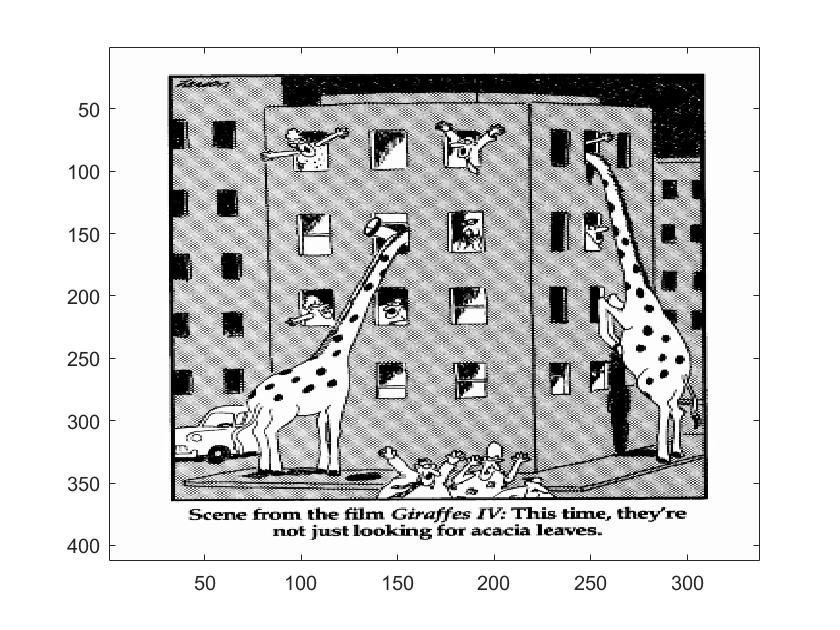
\includegraphics[scale=0.35]{imfiltree_reduite.jpg}
\caption{Image filtrée réduite	}
\label{XX}
\end{center}	\end{figure}


\section{Restauration d'image par filtre de Wiener}
Le but de cette partie est d'atténuer la dégradation (ici le flou) d'une image, par filtrage inverse. On va pour cela utiliser le filtre de Wiener : 
\[
	W(u,v) = \frac{1}{H(u,v)} * \frac{|H(u,v)|^2}{|H(u,v)|^2+\dfrac{P_b(u,v)}{P_i (u,v)}}	
\]

où $H(u,v)$ modélise la translation à l'origine du flou, et $P_i(u,v)$ ainsi que $P_b(u,v)$ sont deux spectres de puissance. $P_i(u,v)$ sera déterminé à partir d'une image de référence $i_r(x,y)$ et $P_B(u,v)$ est approximé par le spectre de puissance du bruit $b(x,y)$ qui apparaît lors du passage de $d_R(x,y)$ (l'image de référence produit de convolution le filtre $H$) à $|d_R(x,y)|$.

Pour la dégradation, on modélise une translation de 17 pixels sur 3 de hauteur.


\begin{figure}[H]	\begin{center}
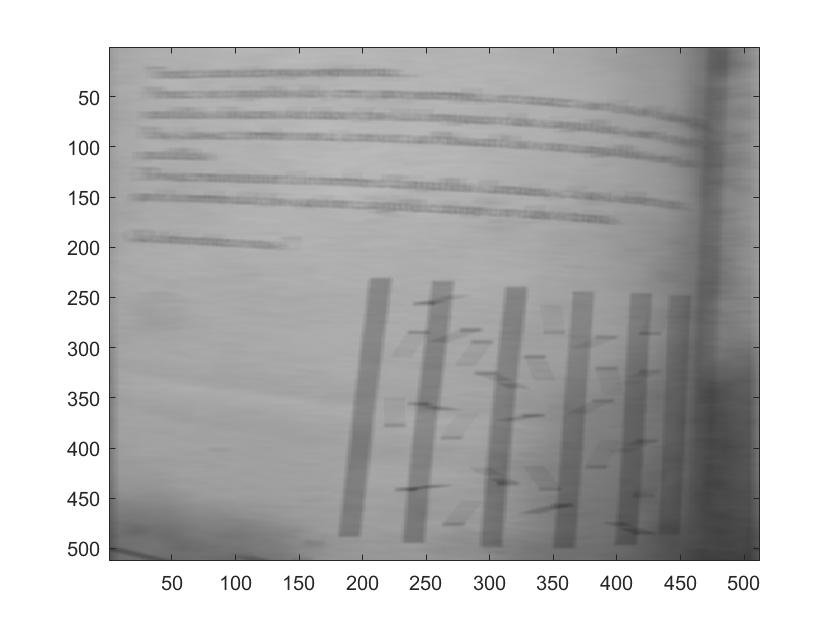
\includegraphics[scale=0.35]{im_floue.jpg}
\caption{L'image originale, floue}
\label{XX}
\end{center}	\end{figure}

\begin{figure}[H]	\begin{center}
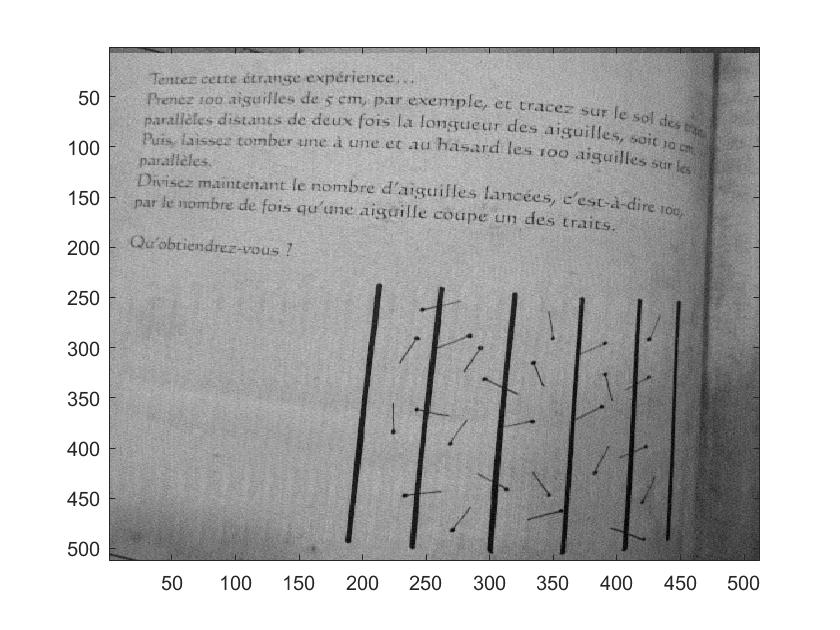
\includegraphics[scale=0.35]{im_restauree.jpg}
\caption{L'image restaurée}
\label{XX}
\end{center}	\end{figure}

On peut donc maintenant lire le texte : 
\textit{\\Tentez cette étrange expérience:\\
Prenez 100 aiguilles de 5cm, par exemple, et racez sur le sol des traits parrallèles distants de deux fois la longueur des aiguilles sur les parrallèles.\\
Divisez maintenant le nombre d'aiguilles lancées, c'est à dire 100, par le nombre de fois qu'une aiguille coupe un des traits.}

\end{document}